\documentclass[11pt]{beamer}
\usepackage[english]{babel}
\usepackage[T1]{fontenc}
\usepackage[utf8]{inputenc}
\usepackage{sourcesanspro}
\usepackage{sourcecodepro}
\usepackage{euler}
\usepackage[normalem]{ulem}
\usepackage{natbib}
\usepackage{apalike}
% \usepackage{bibentry}
% \usepackage{enumitem}
\usepackage[font={scriptsize},labelfont={scriptsize}]{caption}
\usepackage{lmodern,tgtermes,tabularx,ragged2e}
% \newcolumntype{Y}{>{\arraybackslash\RaggedRight}X}
% \newcolumntype{P}[1]{>{\arraybackslash\RaggedRight}p{#1}}
\usepackage{hhline}
\usepackage{booktabs}
\usepackage{array}
\newcolumntype{L}[1]{>{\raggedright\let\newline\\\arraybackslash\hspace{0pt}}m{#1}}
\newcolumntype{C}[1]{>{\centering\let\newline\\\arraybackslash\hspace{0pt}}m{#1}}
\newcolumntype{R}[1]{>{\raggedleft\let\newline\\\arraybackslash\hspace{0pt}}m{#1}}
\usepackage{makecell}
\usepackage{pdfpages}
% \usepackage[overlay,absolute]{textpos}
%   \setlength{\TPHorizModule}{1mm}
%   \setlength{\TPVertModule}{1mm}
\usepackage{graphicx}

% \nobibliography*
\setcitestyle{authoryear,comma,square,aysep={},yysep={}}
% \setbeameroption{hide notes}
% \setbeameroption{notes on second screen=right}
% \setbeameroption{use timer}
% \setbeameroption{use timer countdown=30}

\usetheme{inria}
%\usepackage{helvet}
\AtBeginSection[]{
  \begin{frame}[plain]
    \partpage
  \end{frame}
}
\newcommand{\inriaswitchcolors}[1]{%
\pgfaliasimage{figfootline}{figfootline-#1}% !!!
\pgfaliasimage{figbackground}{figbackground-#1}% !!!
\pgfaliasimage{figbackground}{figbackground-#1}% !!!
}
\setbeamertemplate{blocks}[rounded][shadow=true]
\setbeamercolor{block title}{fg=white,bg=inriaRed1}
\setbeamerfont{block title}{parent=frametitle,size=\small}
\setbeamerfont{section in toc}{parent=structure, size=\large}

% %remove the icon
% \setbeamertemplate{bibliography item}{}

% %remove line breaks
% \setbeamertemplate{bibliography entry title}{}
% \setbeamertemplate{bibliography entry location}{}
% \setbeamertemplate{bibliography entry note}{}

\usepackage{listings}
\usepackage{amsmath,amssymb}
% \usepackage{courier}

\usepackage{tikz}
\usepackage{tikz-cd}
\usetikzlibrary{decorations.pathreplacing,angles,quotes}
\usetikzlibrary{positioning}
\usetikzlibrary{shapes.geometric}
\usetikzlibrary{calc}
\usetikzlibrary{arrows,patterns}
\usetikzlibrary{intersections}
\usetikzlibrary{tikzmark,fit,shapes.geometric}

\definecolor{myviolet}{rgb}{0.6,0.0,0.65}
\definecolor{myblue}{rgb}{0.1,0.0,0.8}
\definecolor{mygreen}{rgb}{0.1,0.8,0.0}
\definecolor{myred}{rgb}{0.8,0.0,0.0}

\definecolor{dkblue}{rgb}{0,0.1,0.5}
\definecolor{lightblue}{rgb}{0,0.5,0.5}
\definecolor{dkgreen}{rgb}{0,0.4,0}
\definecolor{dk2green}{rgb}{0.4,0,0}
\definecolor{dkviolet}{rgb}{0.6,0,0.8}
\definecolor{shadethmcolor}{rgb}{0.9, 0.9,1}

\let\L=\lstinline
\def\lstlanguagefiles{defManSSR.tex}
\lstset{language=SSR}
\lstset{basicstyle=\footnotesize\ttfamily,breaklines=true}
\lstset{framextopmargin=50pt,frame=bottomline}
\lstset{moredelim=[is][\color{red}\bfseries\ttfamily\underbar]{|*}{*|}}
\lstset{moredelim=[is][\color{blue}\bfseries\ttfamily]{/*}{*/}}

\def\mathcomp{{\small\textsc{Mathematical Components}}}
\def\mydef#1{{\sl #1}}
\def\myem#1{{\bf\sl \color{red}{#1}}}
% \def\myem#1{\emph{#1}}

\newcommand{\cvg}[2]{#1 \rightarrow #2}
\newcommand{\abs}[1]{\left\lvert #1 \right\rvert}
\newcommand{\norm}[1]{\left\lVert #1 \right\rVert}
\newcommand{\scal}[2]{\left\langle #1, #2 \right\rangle}
\newcommand\IR{\ensuremath{\mathbb{R}}}
\newcommand\IC{\ensuremath{\mathbb{C}}}
\newcommand\nat{\ensuremath{\mathbb{N}}}
\newcommand\IN{\nat}

\renewcommand{\leq}{\leqslant}

\def\eps{\varepsilon}
\def\lip{LaSalle's invariance principle}
\def\o{\circ}
\def\coq{{\sc Coq}}
\def\ssr{{\sc SSReflect}}
\def\mathcomp{{\sc Mathematical Components}}
\def\coquelicot{{\sc Coquelicot}}
\def\isahol{{\sc Isabelle/HOL}}
\def\hol4{{\sc HOL4}}
\def\hollight{{\sc HOL Light}}
\def\lean{{\sc Lean}}
\def\pvs{{\sc PVS}}
\def\mizar{{\sc Mizar}}
\def\analysis{{\sc Mathematical Components Analysis}}
\def\plim{\Gamma^{+}}
\def\loc{\textrm{locally}}
\def\ball{\textrm{ball}}

\def\us{\char`\_}

\def\newterm#1{{\sl #1}} % to introduce new terms such as ``entourage'', etc.
\def\eg{\textit{e.g.}} % NB(rei): btw, the lncs authors' instructions uses the american convention (``e.g.,'' in roman)
\def\ie{\textit{i.e.}} % NB(rei): for uniformity (there was one with \em instead of \it)
\def\subset{\subseteq}
\def\supset{\supseteq}

% \makeatletter
% \renewenvironment{table}%
%   {\renewcommand\familydefault\sfdefault
%    \@float{table}}
%   {\end@float}
% \makeatother

\newcommand\doubleRule{\toprule\toprule}
\newcommand\doublerule{\toprule\specialrule{\heavyrulewidth}{\doublerulesep}{0.95em}}

\newcommand\coqPR[1]{\coq{} PR \href{https://github.com/coq/coq/issues/#1}{\##1}}
\newcommand\coqIssue[1]{\coq{} Issue \href{https://github.com/coq/coq/issues/#1}{\##1}}

\begin{document}

\title[Hierarchy Builder]{{Hierarchy Builder:}\\ {Algebraic
    hierarchies} \\ {made easy} {in {\sc Coq} with {\sc Elpi}}}
\subtitle{FSCD 2020}

\author[\underline{Cohen}, Sakaguchi, Tassi]{
  \underline{Cyril Cohen \textit{(Inria)}}, Kazuhiko Sakaguchi, Enrico
Tassi}

% \institute[]{\inst{1} Inria, France, \inst{2} University of Tsukuba,
% Japan}

\date{June 2nd, 2020}

\begin{frame}
\titlepage
\end{frame}

\begin{frame}[fragile]
  \frametitle{Structures in Mathematics}

  \begin{itemize}
  \item A \textbf{carrier} in Set / Type,
  \item A set of \textbf{constants} in the carrier, and \textbf{operations},
  \item Proofs of the \textbf{axioms} of the structure
  \end{itemize}

  \pause

\begin{lstlisting}
Record is_ring R := mk_ring {
    zero : R; add : R -> R -> R; opp : R -> R;
    one : R;  mul : R -> R -> R;
    addrA : associative add;
    addrC : commutative add;
    add0r : left_id zero add;
    addNr : left_inverse zero opp add;
    mulrA : associative mul;
    mul1r : left_id one mul;
    mulr1 : right_id one mul;
    mulrDl : left_distributive mul add;
    mulrDr : right_distributive mul add;
  }.
\end{lstlisting}

\end{frame}


\begin{frame}
  \frametitle{Implementations in DTT (unbundled classes)}



\end{frame}


\begin{frame}
  \frametitle{Implementations in DTT (semi-bundled classes)}



\end{frame}

\begin{frame}
  \frametitle{Implementations in DTT (bundled record)}



\end{frame}

\begin{frame}
  \frametitle{Implementations in DTT (packed classes)}



\end{frame}

\begin{frame}
  \frametitle{Implementations in proof assistants}

  A variety of representations:

  % more details comming
  \begin{itemize}
  \item {\sc Coq/Mathcomp}:     Classes packed in (canonical) structures
  \item {\sc Coq/Math-Classes}: Fully unbundled (typeclass) records $+$
                                special case for varieties.
  \item {\sc Lean/Mathlib}:     Variably-bundled (typeclass) records.
  \item {\sc Agda}:             bundled and semi-bundled records.
  \end{itemize}
  \vfill
  \pause

  Many other possibilities:
  \begin{itemize}
  \item Modules a la Ocaml \emph{(not first class!)},
  \item Fully-bundled typeclasses \emph{(bad!)},
  \item Telescopes \emph{(bad!)},
  \item Records without inference \emph{(tedious!)}, ...
  \end{itemize}
  \vfill
  \pause

\center{  \textbf{Representations work hand in hand with an inference
  mechanism.}}

\end{frame}


\begin{frame}
  \frametitle{Inference of structures}

  \begin{itemize}
  \item {\sc Coq/Mathcomp}:     canonical instances $+$ coercions $+$ checker
  \item {\sc Coq/Math-Classes}: typeclass instances $+$ hint extern
  \item {\sc Lean/Mathlib}:     typeclass instances $+$ linter
  \item {\sc Agda}:             \L{open} and renaming directives
  \end{itemize}

  \vfill
  \pause
  None of these encoding are straightforward, they all need
  expert knowledge or checkers/linters, and additionally

  \begin{itemize}
  \item Some encodings are unnecessarily verbose,
  \item Some known design problems might be detected too late
    (e.g. priority of instance, typeclass indexing, forgetful
    inheritance, etc)
  \end{itemize}

  % TODO: maybe insert here showing various encoding artifacts

  \vfill
  \pause
  \center{\textbf{Hierarchy Builder provides a DSL!}}
\end{frame}


\begin{frame}
  \frametitle{Hierarchies in formalization}

  Purpose:
  \begin{itemize}
  \item factor theorems across instances, using the \textbf{theory} of
    each structure,
  \item \textbf{automatically find} which structures hold on which types.
  \end{itemize}

  \pause
  \vfill

  Requirements:
  \begin{itemize}
  \item declare a \textbf{new instance},
  \pause
  \item declare a \textbf{new structure}
    \begin{itemize}
    \item above, below or in the middle
    \item handle diamonds (e.g. monoid, group, commutative or not),
    \item by amending existing code, or not,
    \end{itemize}
  \pause
  \item \textbf{predictability} of inferred instance,
  \pause
  \item \textbf{robustness} of user code with regard to \textit{new declarations}.
  \end{itemize}

\end{frame}

\begin{frame}
  \frametitle{Hierarchy Builder in theory}

  \begin{enumerate}
  \item \textbf{Hierarchy Builder provides a DSL to generates/extends a
      hierarchy from minimal input.}
    \vfill
  \item \textbf{Hierarchy Builder lets you amend a hierarchy without
      breaking your code.}
  \end{enumerate}

  \vfill

  That way, Hierarchy Builder is fully in control of the design
  patterns used throughout your library.
\end{frame}


\begin{frame}
  \frametitle{Hierarchy Builder in practice}

  \begin{itemize}
  \item Hierarchy Builder generates/extends a hierarchy using \mathcomp{}
    packed class methodology.
    \vfill
  \item Hierarchy Builder enforces a discipline of \emph{mixins} and
    \emph{factories} to make client code robust to hierarchy changes.
    \vfill
  \item Hierarchy Builders lets us encode built-in safety measures
    (e.g. detection of overlapping instances)
  \end{itemize}
\end{frame}


\begin{frame}[fragile]
  \frametitle{Structures relating to each other}

  Examples:

  \begin{itemize}
  \item Monoid $\leftarrow$ Group $\leftarrow$ Ring $\leftarrow$ Field
    $\leftarrow$ ...


  \item Euclidean Spaces $\rightarrow$ Normed Spaces $\rightarrow$
    Complete Space $\rightarrow$ Metric Spaces $\rightarrow$ Topological
    Spaces $\rightarrow$ ...

  \end{itemize}

  \pause
  \vfill{}

  \textbf{Going through arrows must be automated.}

  \pause
  \vfill{}

  Arrows represent both
  \begin{itemize}
  \item Extensions: add operations, axioms or combine structures
  \item Entailment/Induction/Deduction/Generalization.
  \end{itemize}

\end{frame}

\begin{frame}
  \frametitle{More examples}

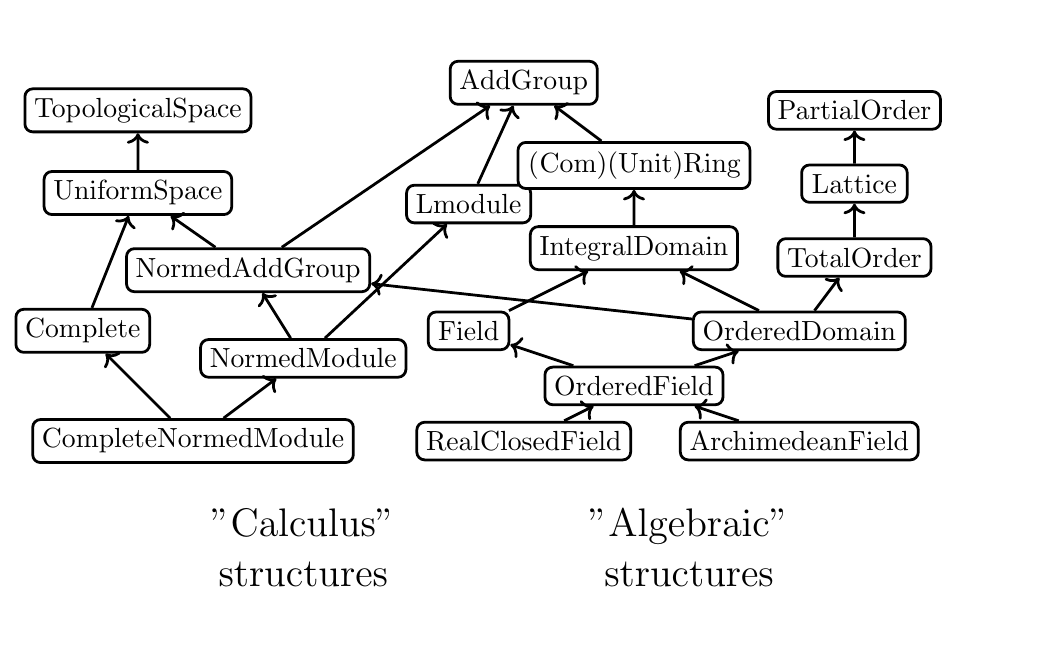
\begin{tikzpicture}[line width=1pt, structure/.style={draw, rounded corners=1mm, fill=white}, new/.style={preaction={fill, white}, pattern=crosshatch dots, pattern color=lightgray}, scale=0.7]
 \useasboundingbox (-6, -.5) rectangle (12, 10.5);
 % Replace `fill` with `pattern`s for the final version.
 %\draw[black!50, pattern=north east lines, pattern color=red!50, rounded corners=15mm] (-7.5, -.5) -- (-7.5, 7) -- (-4, 7) -- (2, 3) -- (2, -.5) -- cycle;
 %\draw[black!50, pattern=north west lines, pattern color=blue!50, rounded corners=15mm] (-8, -.5) -- (2, 4) -- (-4, 8) -- (0, 10) -- (10, 5) -- (10, -.5) -- cycle;
 %
 \node at (-1, 1) {\Large \begin{tabular}{c}''Calculus''\\structures\end{tabular}};
 \node at (6, 1) {\Large \begin{tabular}{c}''Algebraic''\\structures\end{tabular}};
 %
 \node[structure] (PartialOrder)          at (9,  9) {\L+PartialOrder+};
 \node[structure] (Lattice)         at (9,  7.67) {\L+Lattice+};
 \node[structure] (TotalOrder)           at (9,  6.33) {\L+TotalOrder+};
 %
 \node[structure] (AddGroup)             at (3,  9.5) {\L+AddGroup+};
 \node[structure] (Lmodule)              at (2, 7.3) {\L+Lmodule+};
 \node[structure] (Rings)                at (5,  8) {\L+(Com)(Unit)Ring+};
 \node[structure] (IntegralDomain)       at (5,  6.5) {\L+IntegralDomain+};
 \node[structure] (Field)                at (2,  5) {\L+Field+};
 \node[structure] (OrderedDomain)        at (8,  5) {\L+OrderedDomain+};
 \node[structure] (OrderedField)         at (5,  4) {\L+OrderedField+};
 \node[structure] (RealClosedField)      at (3,  3) {\L+RealClosedField+};
 \node[structure] (ArchimedeanField)     at (8,  3) {\L+ArchimedeanField+};
 %
 \node[structure] (TopologicalSpace)          at (-4, 9) {\L+TopologicalSpace+};
 \node[structure] (UniformSpace)              at (-4, 7.5) {\L+UniformSpace+};
 \node[structure] (Complete)             at (-5, 5) {\L+Complete+};
 \node[structure] (NormedAddGroup)       at (-2,  6.1) {\L+NormedAddGroup+};
 \node[structure] (NormedModule)         at (-1, 4.5) {\L+NormedModule+};
 \node[structure] (CompleteNormedModule) at (-3, 3) {\L+CompleteNormedModule+};
 %
 \draw[<-] (PartialOrder) to (Lattice);
 \draw[<-] (Lattice) to (TotalOrder);
 \draw[<-] (TopologicalSpace) to (UniformSpace);
 \draw[<-] (UniformSpace) to (Complete);
 \draw[<-] (UniformSpace) to (NormedAddGroup);
 \draw[<-] (Complete) to (CompleteNormedModule);
 \draw[<-] (Lmodule) to (NormedModule);
 \draw[<-] (NormedAddGroup) to (NormedModule);
 \draw[<-] (NormedModule) to (CompleteNormedModule);
 \draw[<-] (AddGroup) to (Lmodule);
 \draw[<-] (AddGroup) to (NormedAddGroup);
 \draw[<-] (AddGroup) to (Rings);
 \draw[<-] (Rings) to (IntegralDomain);
 \draw[<-] (IntegralDomain) to (OrderedDomain);
 \draw[<-] (NormedAddGroup) to (OrderedDomain);
 \draw[<-] (TotalOrder) to (OrderedDomain);
 \draw[<-] (IntegralDomain) to (Field);
 \draw[<-] (Field) to (OrderedField);
 \draw[<-] (OrderedDomain) to (OrderedField);
 \draw[<-] (OrderedField) to (RealClosedField);
 \draw[<-] (OrderedField) to (ArchimedeanField);

 % \draw[opacity=.5, black, fill=red!50, rounded corners=15mm] (-7.5, -.5) -- (-7.5, 7) -- (-4, 7) -- (2.5, 3) -- (2, -.5) -- cycle;
 % \draw[opacity=.5, black, fill=blue!50, rounded corners=15mm] (-8, -.5) -- (1.5, 4) -- (-4.3, 8) -- (0, 10) -- (10.5, 5.5) -- (10, -.5) -- cycle;
 \end{tikzpicture}

\end{frame}

\begin{frame}
  \frametitle{Structure extension vs Structure entailment}
  \begin{columns}
    \begin{column}{0.5\textwidth}
      \begin{center}
        {\bf \emph{Structure extension}}
      \end{center}
    \end{column}
    \begin{column}{0.5\textwidth}
      \begin{center}
        {\bf \emph{Structure extension}}
      \end{center}
    \end{column}
  \end{columns}
  \vfill
  \begin{columns}
    \begin{column}{0.5\textwidth}
      \begin{itemize}
      \item \textbf{Compositional}: no need to start from scratch every time.
        (E.g. the product of two groups is a group)
        \pause\vfill
      \item \textbf{Noisy}: changes the internal definition of a structure.
        (E.g. defining a commutative monoid from a monoid, one gets an unnecessary axiom),
        \pause\vfill
      \item \textbf{Non-robust}: breakage of user code when adding new
        intermediate structures, \pause\vfill
      \end{itemize}
    \end{column}
    \begin{column}{0.5\textwidth}
      \begin{itemize}
      \item \textbf{More flexible}: no need to cut structures
        into small bits,
        \pause\vfill
      \item \textbf{Robust}: lets us fix the operations and axioms
        once and for all.
        \pause\vfill
      \item \textbf{Not suitable for inference}: Major breakage when
        arbitrary entailment is automatic. (cf IJCAR \emph{Formalizing
          functional analysis structures in dependent type theory)}
        \pause\vfill
      \end{itemize}
    \end{column}
  \end{columns}
  \vfill

\end{frame}


\begin{frame}
  \frametitle{HB Design}

  The best of two the worlds:
  \begin{itemize}
  \item \textbf{Extension}, through \emph{mixins} for \textbf{internal declaration} and
    \textbf{automatic inference}

  \item \textbf{Entailment}, through \emph{factories} for any other use.

    Factories require mixins and can produces others.
    (e.g. a full axiomatic can provide all the pieces)
  \end{itemize}
  \vfill

  Five commands:
  \begin{enumerate}
  \item \L{HB.mixin     Record axioms T := \{..\}.}
  \item \L{HB.factory   Record axioms T := \{..\}.}
  \item \L{HB.builder   Context       T (f : axioms T). ... HB.end.}
  \item \L{HB.structure Definition    S := \{ T & axioms T \}}
  \item \L{HB.instance  Definition    f := Axioms X ...}
  \end{enumerate}
  \vfill
  \begin{center}
    \url{https://github.com/math-comp/hierarchy-builder}
  \end{center}

\end{frame}

\begin{frame}[fragile]
  \frametitle{A very short example}

\begin{lstlisting}
HB.mixin Record is_monoid (M : Type) := {
  zero : M;
  add : M -> M -> M;
  addrA : associative add;   (* add is associative. *)
  add0r : left_id zero add;  (* zero is the neutral *)
  addr0 : right_id zero add; (*    element wrt add. *)
}.
HB.structure Definition Monoid := { M & is_monoid M }.

HB.instance Definition Z_Monoid_axioms : is_monoid Z :=
  is_monoid.Build Z 0%Z Z.add
    Z.add_assoc Z.add_0_l Z.add_0_r.
\end{lstlisting}
  \vfill

  See a full demo during the Coq workshop.
\end{frame}

\begin{frame}[fragile]
  \frametitle{Breaking down monoid}

  We split the monoid structure into a semi-group and a monoid
  \begin{lstlisting}
HB.mixin Record is_semigroup (S : Type) := {
  add : S -> S -> S;
  addrA : associative add;   (* add is associative. *)
}.
HB.structure Definition SemiGroup :=
  { S & is_semigroup S }.

HB.mixin Record monoid_of_semigroup (M : Type) := {
  zero : M;
  add0r : left_id zero add;  (* zero is the neutral *)
  addr0 : right_id zero add; (*    element wrt add. *)
}.
HB.structure Definition Monoid :=
  { M & monoid_of_semigroup M }.
\end{lstlisting}
\center{\textbf{But we must provide \L{is_monoid} again.}}
\end{frame}

\begin{frame}[fragile]
  \frametitle{Recovering \L{is_monoid}}

  It becomes a \emph{factory}.
\begin{lstlisting}
HB.factory Record is_monoid (M : Type) := {
  zero : M;
  add : M -> M -> M;
  addrA : associative add;
  add0r : left_id zero add;
  addr0 : right_id zero add;
}.

HB.builder Context (M : Type) (f : is_monoid M) :=
  HB.instance Definition is_monoid_semigroup :
    is_semigroup M := ...
  HB.instance Definition is_monoid_monoid :
    monoid_of_semigroup M := ...
HB.end
\end{lstlisting}
\end{frame}

\begin{frame}
  \frametitle{Meta programming in {\sc Coq-ELPI}}

\end{frame}

\begin{frame}
  \frametitle{Conclusion}

  \begin{itemize}
  \item High-level commands to declare structures and instances, \\
    easy to use.
    \vfill
  \item Predictable outcome of inference,
    \vfill
  \item Takes into account the evolution of knowledge
    \begin{itemize}
    \item which is formalized, and
    \item which the user has.
    \end{itemize}
    The two knowledge do not need to be correlated.
    \vfill
  \item Robustness with regard to new declaration \emph{and even changes of
    internal implementation}.
  \end{itemize}

  \vfill\pause
  Also, \textsc{Coq-ELPI} turned out to be a very comfortable
  meta-programming language for this.

\end{frame}

\begin{frame}
  \frametitle{Future work on Hierarchy Builder}
  \begin{itemize}
  \item Adding support for parameters. (debugging phase in progress)
    \vfill
  \item Detecting and fixing competing inheritance paths.
    \vfill
  \item Generating hierarchies of morphisms from structures.
    \vfill
  \item Generating hierarchies of subobjects from structures.
    \vfill
  \item Supporting multiple instances on the same carrier.
    \vfill
  \item Replacing all uses in math-comp and extensions.
    \vfill
  \item Get better error messages.
  \end{itemize}
\end{frame}

\end{document}
